\section{Estudo Exprimental}

Para alcançar o objetivo de identificar quantos warnings das ferramentas CogniCrypt e CryptoGuard advém ou não de uma biblioteca externa, adotamos a abordagem GQM (Goal, Question, Metric), conforme descrito a seguir:

\subsection{Objetivo}

Identificar a quantidade de \textit{warnings} das ferramentas CogniCrypt e CryptoGuard que advém de bibliotecas externas. 

\subsubsection{Questões de Pesquisa}
Definimos as seguintes perguntas baseadas nos dados coletados:

\begin{itemize}
\item \textbf{RQ1:} Qual é a quantidade de \textit{warnings} no \textit{dataset} de aplicativos Android analisados pelas ferramentas CogniCrypt e CryptoGuard?

\item \textbf{RQ2:} Qual é a quantidade de \textit{warnings} que pertencem a bibliotecas externas nos aplicativos Android do \textit{dataset} analisado pelas ferramentas CogniCrypt e CryptoGuard?

\end{itemize}

\subsubsection{Métricas}
Para responder às questões RQ1 e RQ2  as seguintes métricas foram estabelecidas:

\begin{itemize}
\item \textbf{M1: Número total de \textit{warnings} detectados pela ferramenta CogniCrypt.} \
\item \textbf{M2: Número total de \textit{warnings} detectados pela ferramenta CryptoGuard.} \
\item \textbf{M3: Número total de \textit{warnings} detectados que pertencem a bibliotecas externas na ferramenta CogniCrypt.} \
\item \textbf{M4: Número total de \textit{warnings} detectados que pertencem a bibliotecas externas na ferramenta CryptoGuard.} \
\end{itemize}

\section{Metodologia do Estudo}

Para conseguir essas métricas e responder às questões de pesquisa, a pesquisa foi dividida em várias fases, conforme descrito a seguir:
\begin{figure}[!ht]
  \centering
  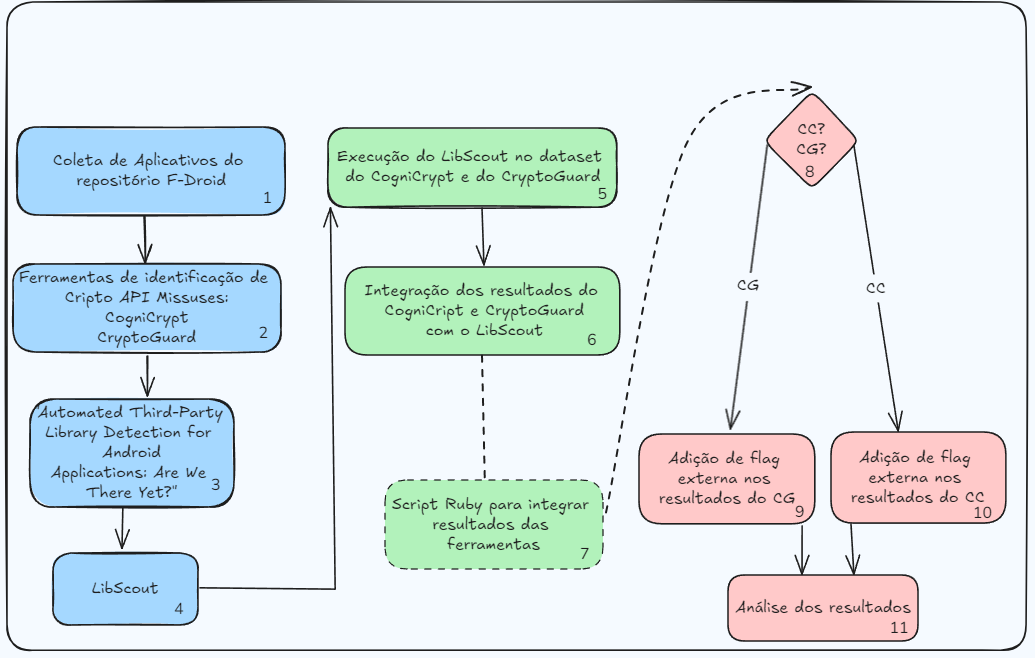
\includegraphics[scale=0.5]{img/research_steps2.png}
  \caption{Fases da pesquisa}
  \label{img: research_steps2}
\end{figure}

\FloatBarrier

\subsection{Seleção de dataset} 

Inicialmente, foi coletado um conjunto de aplicativos Android de código aberto para análise.  O conjunto de dados foi obtido do repositório \href{https://f-droid.org/pt_BR/packages/}{F-Droid}, que contém aplicativos de código aberto disponíveis para download. O dataset foi separado em categorias: Connectivity, Finances, Internet, SMS e System. O repositório foi escolhido devido à sua natureza de código aberto e à disponibilidade de aplicativos para download. Conforme ilustrado na imagem (\ref{img: research_steps2}), essa etapa corresponde ao primeiro balão azul.

Em seguida, na etapa dois da imagem (\ref{img: research_steps2}),  foram utilizadas as ferramentas CogniCrypt e CryptoGuard para analisar os aplicativos e identificar vulnerabilidades em APIs criptográficas. As ferramentas foram escolhidas devido à sua capacidade de detectar vulnerabilidades em APIs criptográficas e fornecer alertas aos desenvolvedores sobre possíveis problemas de segurança. Ambas as ferramentas foram executadas em um ambiente Docker rodando scripts estruturados para garantir a reprodutibilidade dos resultados. 


\subsubsection{CogniCrypt}

O CogniCrypt foi executado em um ambiente Docker por meio de \textit{scripts}. A versão utilizada foi a \textit{CryptoAnalysis-2.8.0-SNAPSHOT-jar-with-dependencies}. Um trecho do \textit{script} python para a execução em múltiplos aplicativos pode ser visto na imagem (\ref{img: cognicrypt_script}). No código declaramos algumas variáveis de ambiente tais como a localização do .jar do CogniCrypt, as pastas em que se encontram os \textit{apks} e pastas de resultados. O \textit{script} roda em cada um dos aplicativos selecionados via um loop onde executamos o CogniCrypt com alguns argumentos necessários como a quantidade de memória que será utilizada e os caminhos necessários para rodar o experimento.
Podemos ver um exemplo do resultado em json do CogniCrypt nas imagens em anexo (\ref{img: cognicrypt_output}) (\ref{img: cognicrypt_output2}). No trecho apresentado nas duas imagens, temos para o aplicativo Ademar.bitac\_5 os \textit{warnings} de \textit{cripto api missuses}. Nesses resultados, temos o parâmetro \textit{FullyQualifiedLogicalName} o qual indica o caminho lógico em que se encontra a vulnerabilidade.

\subsubsection{CryptoGuard}

A execução da ferramenta CryptoGuard foi semelhante a do CogniCrypt. A ferramenta foi executada em um ambiente Docker por meio de \textit{scripts}. A versão utilizada foi a \textit{CryptoGuardCVER04.05.03}. Um trecho do \textit{script} python para a execução em múltiplos aplicativos pode ser visto na imagem (\ref{img: cryptoguard_script}). No código apresentado, podemos ver de forma semelhante à declaração das variáveis de ambiente que serão utilizadas e um loop para iterar em cada aplicativo do dataset. O loop executa o CryptoGuard com alguns argumentos tais como a quantidade de memória utilizada e os caminhos relativos que serão utilizados.
Um exemplo de resultado do CryptoGuard pode ser visto na imagem em anexo (\ref{img: cryptoguard_output}). O resultado da ferramenta é um json que apresenta o comando utilizado para execução, o caminho completo do aplicativo, outras propriedades e o mais importante o trecho de \textit{Issues} que traz consigo os \textit{warnings} de \textit{cripto api missuses} e o \textit{FullPath} que indica o caminho lógico em que se encontra a vulnerabilidade.

\subsubsection{LibScout}

Na etapa três da imagem (\ref{img: research_steps2}), para identificar as bibliotecas externas, fizemos uma análise da literatura e através do estudo realizado por \cite{api_tpl_zhang}, identificamos o LibScout como uma ferramenta eficaz para identificar bibliotecas em aplicativos Android. O LibScout foi escolhido devido à sua capacidade de identificar bibliotecas em aplicativos Android e fornecer informações detalhadas sobre as bibliotecas encontradas. O estudo cita outras ferramentas que poderiam ser utilizadas, como o LibRadar, LibID, libPecker. O LibRadar foi um dos aplicativos inicialmente considerados para podermos comparar com os resutlados do LibScout, no entanto, o número de bibliotecas externas encotradas em um subset dos quais já sabiamos os resultados não foi suficiente. O LibRadar compara os resultados da investigação com um dataset base, o qual não foi atualizado nos últimos 7 anos. Cada uma das ferramentas destacadas no paper de Zhang tem suas limitações, como a falta de atualizações de datasets, tempo exagerado para análise de apenas um aplicativo, baixa confiabilidade nos resultados. De todas as métricas descritas no artigo, o LibScout foi a que apresentava resultados mais confiáveis em tempo hábil para análise de um grande número de aplicativos. Assim, a etapa quatro da imagem (\ref{img: research_steps2}) representa a escolha do libScout. 

Na etapa cinco da imagem (\ref{img: research_steps2}), para a execução do LibScout, foi necessário instalar o Android SDK, além de configurar o ambiente de desenvolvimento. O LibScout também foi executado em um ambiente docker através de scripts estruturados para garantir a reprodutibilidade dos resultados. Foi utilizado a versão 2.3.2. Um exemplo do script utilizado para a execução do LibScout pode ser visto na imagem em anexo (\ref{img: libscout_script}). De forma semelhante às ferramentas anteriores, o script inclui a declaração das variáveis de ambiente e um loop para a execução do LibScout. Um argumento relevante na execução do LibScout, além dos caminhos de arquivos, é a diretiva \textit{-a}. Essa diretiva é utilizada para diferenciar o código do aplicativo do código do framework Android, sendo necessário o Android SDK (jar) para essa distinção. Um exemplo de resultado do LibScout para o aplicativo Ademar.bitac\_5 pode ser visto nas imagens em anexo (\ref{img: libscout_output}) e (\ref{img: libscout_output2}). O trecho da primeira imagem contém o mapeamento de todas as bibliotecas alcançáveis do aplicativo. Elas são acompanhadas da tag \textit{LibraryIdentifier}. Na segunda imagem temos os resultados do \textit{ProfileMatch} que traz as bibliotecas externas do aplicativo. O arquivo de saída é em formato .log. 

\subsection{Integração dos resultados do CogniCript e CryptoGuard com o LibScout} 
A etapa seis da imagem (\ref{img: research_steps2}), integramos os resultados do LibScout aos contextos das ferramentas CryptoGuard e CogniCrypt. Essa integração permitiu uma análise mais detalhada e contextualizada das vulnerabilidades encontradas, especialmente em bibliotecas externas. As etapas seguintes da imagem (\ref{img: research_steps2}) estão descritas a seguir.

A integração se deu por meio de scripts que cruzam os resultados das ferramentas de análise estática com os resultados do LibScout. A lógica utilizada para adicionar a flag de biblioteca extena nos resultados do CogniCrypt pode ser observada na imagem em anexo (\ref{img: integration_script_cogni}). No laço principal, após carregar o resultado do libscout e do cognicrypt nós verificamos se existe um casamento entre algum dos ProfileMatch com algum dos warnings com o FullyQualifiedLogicalName que sejam iguais. Caso exista, o warning é clasificado como advindo de uma biblioteca externa. A estratégia é semelhante para o CryptoGuard (\ref{img: integration_script_crypto}), exceto que o casamento é feito com o FullPath. 

\subsection{Análise de dados} 

Durante a análise, geramos gráficos e tabelas para ilustrar a distribuição de \textit{warnings} e a prevalência de vulnerabilidades. Os resultados foram gerados utilizando scripts para contar o número de \textit{warnings} e bibliotecas externas identificadas. A imagem em anexo (\ref{img: output_script}) exemplifica parte da lógica do script para gerar os dados para análise. O script em questão gera um csv com a quantidade de bibliotecas analisadas, bibliotecas nativas e bibliotecas externas utilizando os resultados da integração das ferramentas.


\section{Resultados}

\subsection{RQ1. Quantidade de warnings encontrados pelas ferramentas CogniCrypt e CryptoGuard}

Foram analisados 260 aplicativos de 6 diferentes categorias do repositório de aplicativos de código aberto F-Droid. A execução do CogniCrypt reportou 195 \textit{warnings} de uso indevido de criptografia, enquanto o CryptoGuard reportou 298. A tabela abaixo mostra a quantidade de aplicativos analisados por categoria e a quantidade de \textit{warnings} reportados por cada ferramenta.

\begin{table}[!htbp]
  \centering
  \begin{tabular}{|c|c|c|c|}
  
    \textbf{Categoria}   & \textbf{Número de Aplicativos}   &  \textbf{CogniCrypt}     &  \textbf{CryptoGuard} \\ 
     Connectivity           & \num{58}                         &  \num{20}                    & \num{3}                     \\
Finances                & \num{90}                         &  \num{25}                    & \num{2}                     \\
Internet                 & \num{39}                         &  \num{7}                      &     \num{0}                  \\
Sms-Phone            & \num{18}                         &  \num{10}                     &     \num{2}                 \\
System                  & \num{55}                        &   \num{34}                    &     \num{0}                  \\
\textbf{Total}        & \num{260}                      &   \num{96}                  &     \num{7}                   \\
\end{tabular}
    
  \caption{Aplicativos por categoria sem warning das ferramentas CogniCrypt e CryptoGuard}
\label{AplicativosSemWarning}
\end{table}

Como visto, o número de aplicativos sem \textit{warnings} no CogniCrypt é bem maior do que no CryptoGuard. A categoria Sistema é a que apresenta a maior diferença entre eles, com \num{34} aplicativos. As categorias Conectividade e Finanças também têm um número elevado de aplicativos sem \textit{warnings}, \num{20} e \num{25}, respectivamente.

Apesar disso, o número de \textit{warnings} encontrados pelo CogniCrypt é maior do que no CryptoGuard, conforme descrito na tabela abaixo.

\begin{table}[!htbp]
  \centering
  \begin{tabular}{|c|c|c|c|}
    \hline
    \textbf{Categoria}   & \textbf{CogniCrypt (a)}   &  \textbf{CryptoGuard (b)}     &  \textbf{Diferença (a - b)} \\ 
    \hline
    Connectivity           & \num{1768} (\num{19.10}\%)  &  \num{1124} (\num{25.48}\%)  & \num{644} (\num{13.29}\%) \\
    Finances                & \num{3087} (\num{33.35}\%) & \num{1687} (\num{38.25}\%) & \num{1400} (\num{28.90}\%)\\
    Internet                 & \num{3407} (\num{36.81}\%) & \num{916} (\num{20.77}\%) & \num{2491} (\num{51.41}\%)\\
    Sms-Phone            & \num{428} (\num{4.62}\%) & \num{171} (\num{3.88}\%) & \num{257} (\num{5.30}\%)\\
    System                  & \num{566} (\num{6.11}\%) & \num{513} (\num{11.63}\%) & \num{53} (\num{1.09}\%)\\
    \hline
    \textbf{Total}          & \num{9256} (\num{100.00}\%) & \num{4411} (\num{100.00}\%) & \num{4845} (\num{100.00}\%)\\
    \hline
  \end{tabular}
    
  \caption{Warnings encontrados nas ferramentas CogniCrypt e CryptoGuard}
  \label{AplicativosComWarning}
\end{table}

Como podemos observar na tabela acima, o CogniCrypt conseguiu encontrar \num{9256} \textit{warnings}, enquanto o CryptoGuard encontrou \num{4411} \textit{warnings}. A diferença numérica é de \num{4845} (ou \num{109.84}\%) \textit{warnings} entre as duas ferramentas. As categorias de Finanças e Internet concentraram \num{70.2}\% (\num{6494}) dos \textit{warnings} do CogniCrypt, enquanto as categorias de Finanças e Conectividade concentraram \num{63.7}\% (\num{2811}) dos \textit{warnings} do CryptoGuard. A maior diferença entre os \textit{warnings} encontrados foi notada nas categorias Internet (\num{2491}) e Finanças (\num{1400}), representando \num{80.3}\% de diferença.

\subsection{RQ2.  Qual é a quantidade de \textit{warnings} que pertencem a bibliotecas externas nos aplicativos Android do \textit{dataset} analisado pelas ferramentas CogniCrypt e CryptoGuard?}

Em cada categoria, serão exibidos os resultados relativos ao número de aplicativos com alertas de vulnerabilidade, para cada ferramenta utilizada. As tabelas a seguir apresentam os resultados dessas integrações.

\subsubsection{CogniCrypt}

\begin{table}[!htbp]
  \centering
  \small
  \begin{tabular}{|c|c|c|c|}
  
\textbf{CC/Connectivity}   & \textbf{Total Warnings (a)}   &   \textbf{External Libraries (b)} &  \textbf{Native Libraries (a-b)} \\ 
Média                      & \num{21.9}              & \num{2.4}                                        & \num{17.1}                                                    \\
Desvio Padrão              & \num{43.8}              & \num{6.1}                                        & \num{42.8}                                 \\                    
Variância                  & \num{1919.8}            & \num{38.2}                                       & \num{1831.9}         \\                                           
\end{tabular}
    
  \caption{Resultados da integração do CogniCrypt com o LibScout na categoria Connectivity}
\label{table: AplicativosComWarningCCC}
\end{table}


\begin{table}[!htbp]
  \centering
  \small
  \begin{tabular}{|c|c|c|c|}
  
\textbf{CC/Finances}   & \textbf{Total Warnings (a)}   &  \textbf{External Libraries (b)} &  \textbf{Native Libraries (a-b)} \\ 
Média                      & \num{46.4}          & \num{7.5}                                         & \num{35.9}                                                    \\
Desvio Padrão              & \num{132.06}          & \num{41.8}                                        & \num{126.07}          \\                                          
Variância                  & \num{17439.9}       & \num{1747.7}                                      & \num{15895.3}    \\                                                
\end{tabular}
    
  \caption{Resultados da integração do CogniCrypt com o LibScout na categoria Finances}
\label{table: AplicativosComWarningCCF}
\end{table}


\begin{table}[!htbp]
  \centering
  \small
  \begin{tabular}{|c|c|c|c|}
  
\textbf{CC/SMS}   & \textbf{Total Warnings (a)}   &  \textbf{External Libraries (b)} &  \textbf{Native Libraries (a-b)} \\ 
Média                      & \num{11.7}              & \num{1}                                        & \num{8.3}                                                    \\
Desvio Padrão              & \num{31.67}             & \num{3.69}                                        & \num{24.1}   \\                                                 
Variância                  & \num{1003.03}            & \num{12.94}                                       & \num{585.4}             \\                                       
\end{tabular}
    
  \caption{Resultados da integração do CogniCrypt com o LibScout na categoria SMS}
\label{table: AplicativosComWarningCCSMS}
\end{table}


\begin{table}[!htbp]
  \centering
  \small
  \begin{tabular}{|c|c|c|c|}
  
\textbf{CC/System}   & \textbf{Total Warnings (a)}   &  \textbf{External Libraries (b)} &  \textbf{Native Libraries (a-b)} \\ 
Média                      & \num{10.09}              & \num{0.36}                                        & \num{8.79}                                                    \\
Desvio Padrão              & \num{33.01}              & \num{1.28}                                        & \num{31.82}  \\                                                  
Variância                  & \num{1090.2}            & \num{1.66}                                       & \num{1012.5}  \\                                                  
\end{tabular}
    
  \caption{Resultados da integração do CogniCrypt com o LibScout na categoria System}
\label{table: AplicativosComWarningCCS}
\end{table}

Para conectividade (\ref{table: AplicativosComWarningCCC}), a média de \textit{warnings} por aplicativo é de \num{21.9} e a média de \textit{warnings} de biblioteca externas é de \num{2.4}. A quantidade de \textit{warnings} de bibliotecas nativas é de \num{17.1}.

Para finanças (\ref{table: AplicativosComWarningCCF}), a média de \textit{warnings} por aplicativo é de \num{46.4} e a média de \textit{warnings} de biblioteca externas é de \num{7.5}. A quantidade de \textit{warnings} que pertencem a bibliotecas nativas é de \num{35.9}. 

Para SMS (\ref{table: AplicativosComWarningCCSMS}), a média de \textit{warnings} por aplicativo é de \num{11.7} e a média de \textit{warnings} de bibliotecas externas é \num{1}. A quantidade em média de \textit{warnings} que pertecentem a bibliotecas nativas é de \num{8.3}.

Para sistema (\ref{table: AplicativosComWarningCCS}), a média de \textit{warnings} por aplicativo é de \num{10.09} e a média de \textit{warnings} de bibliotecas externas é \num{0.36} A quantidade em média de \textit{warnings} que pertecentem a bibliotecas nativas é de \num{8.79}.

Em todos os exemplos, o desvio padrão e a variância são altos, indicando que os valores estão bem dispersos. Isso é explicado tanto pelas limitações do LibScout quanto pelas limitações do CogniCrypt. O LibScout pode não ter mapeado a biblioteca com \textit{warning} como externa, e o CogniCrypt pode ter encontrado \textit{warnings} em bibliotecas que não foram mapeadas pelo LibScout ou ainda não ter encontrado vulnerabilidade no aplicativo selecionado.

\subsubsection{CryptoGuard}

\begin{table}[!htbp]
  \centering
  \small
  \begin{tabular}{|c|c|c|c|}
    \hline
    \textbf{CG/Connectivity} & \textbf{Total Warnings (a)} & \textbf{External Libraries (b)} & \textbf{Native Libraries (a-b)} \\
    \hline
    Média & \num{15.1} & \num{5.21} & \num{9.22} \\
    Desvio Padrão & \num{25.62} & \num{9.91} & \num{18.7} \\
    Variância & \num{656.6} & \num{98.3} & \num{352.4} \\
    \hline
  \end{tabular}
  \caption{Resultados da integração do CryptoGuard com o LibScout na categoria Connectivity}
  \label{table: AplicativosComWarningCGC}
\end{table}


\begin{table}[!htbp]
  \centering
  \small
  \begin{tabular}{|c|c|c|c|}
    \hline
    \textbf{CG/Finances} & \textbf{Total Warnings (a)} & \textbf{External Libraries (b)} & \textbf{Native Libraries (a-b)} \\
    \hline
    Média & \num{10.45} & \num{4.68} & \num{4.43} \\
    Desvio Padrão & \num{20.71} & \num{10.03} & \num{10.05} \\
    Variância & \num{429.13} & \num{100.72} & \num{101.1} \\
    \hline
  \end{tabular}
  \caption{Resultados da integração do CryptoGuard com o LibScout na categoria Finances}
  \label{table: AplicativosComWarningCGF}
\end{table}


\begin{table}[!htbp]
  \centering
  \small
  \begin{tabular}{|c|c|c|c|}
    \hline
    \textbf{CG/SMS} & \textbf{Total Warnings (a)} & \textbf{External Libraries (b)} & \textbf{Native Libraries (a-b)} \\
    \hline
    Média & \num{9} & \num{2.73} & \num{5.47} \\
    Desvio Padrão & \num{18.72} & \num{5.66} & \num{16.22} \\
    Variância & \num{350.6} & \num{32.08} & \num{263.19} \\
    \hline
  \end{tabular}
  \caption{Resultados da integração do CryptoGuard com o LibScout na categoria SMS}
  \label{table: AplicativosComWarningCGSMS}
\end{table}


\begin{table}[!htbp]
  \centering
  \small
  \begin{tabular}{|c|c|c|c|}
    \hline
    \textbf{CG/System} & \textbf{Total Warnings (a)} & \textbf{External Libraries (b)} & \textbf{Native Libraries (a-b)} \\
    \hline
    Média & \num{7.53} & \num{2.67} & \num{4.2} \\
    Desvio Padrão & \num{16.49} & \num{7.07} & \num{12} \\
    Variância & \num{272.21} & \num{50.07} & \num{146.4} \\
    \hline
  \end{tabular}
  \caption{Resultados da integração do CryptoGuard com o LibScout na categoria System}
  \label{table: AplicativosComWarningCGS}
\end{table}

Para conectividade (\ref{table: AplicativosComWarningCGC}), a média de \textit{warnings} por aplicativo é de \num{15.1} e a média de \textit{warnings} de bibliotecas externas é de \num{5.21}. A quantidade de \textit{warnings} de bibliotecas nativas é de \num{9.22}. 

Para finanças (\ref{table: AplicativosComWarningCGF}), a média de \textit{warnings} por aplicativo é de \num{10.45} e a média de \textit{warnings} de bibliotecas externas é de \num{4.68}. A quantidade de \textit{warnings} de bibliotecas nativas é de \num{4.43}.

Para SMS (\ref{table: AplicativosComWarningCGSMS}), a média de \textit{warnings} por aplicativo é de \num{9} e a média de \textit{warnings} de bibliotecas externas é de \num{2.73}. A quantidade de \textit{warnings} de bibliotecas nativas é de \num{5.47}.

Para sistema (\ref{table: AplicativosComWarningCGS}), a média de \textit{warnings} por aplicativo é de \num{7.53} e a média de \textit{warnings} de bibliotecas externas é de \num{2.67}. A quantidade de \textit{warnings} de bibliotecas nativas é de \num{4.2}. 

Assim como no CogniCrypt, o altos desvios padrão e variância indicam uma dispersão significativa, influenciada pelas limitações do LibScout e do CryptoGuard. O LibScout pode não ter mapeado a biblioteca com \textit{warning} como externa, e o CryptoGuard pode ter encontrado \textit{warnings} em bibliotecas que não foram mapeadas pelo LibScout ou ainda não ter encontrado vulnerabilidade no aplicativo selecionado.

\begin{table}[!htbp]
  \centering
  \small
  \begin{tabular}{|c|c|c|}
    \hline
    \textbf{-} & \textbf{CogniCrypt} & \textbf{Cryptoguard} \\
    \hline
    Total Aplicativos & \num{246} & \num{253} \\
    Total Bibliotecas & \num{6798} & \num{2710}  \\
    Total Bibliotecas Externas & \num{1710} & \num{1149} \\
    Total Bibliotecas Nativas & \num{5088} & \num{1561} \\
    \hline
  \end{tabular}
  \caption{Resultados da integração do CryptoGuard com o LibScout na categoria System}
  \label{table: AplicativosComWarningSummary}
\end{table}

A tabela \ref{table: AplicativosComWarningSummary} mostra um resumo dos resultados obtidos nas categorias analisadas. O CogniCrypt analisou 246 aplicativos, com 6798 bibliotecas, das quais 1710 são externas e 5088 nativas. O CryptoGuard analisou 253 aplicativos, com 2710 bibliotecas, das quais 1149 são externas e 1561 nativas.

Os resultados para a ferramenta CogniCrypt se destacaram em relação aos resultados para o CryptoGuard como podemos ver na imagem em anexo (\ref{img: CCvsCG_Summary}) e a análise proporcional (\ref{img: CCvsCG_Summary2})

\subsubsection{Análise comparativa categorizada entre as ferramentas CogniCrypt e CryptoGuard}

Na categoria de conectividade (\ref{img: CCvsCG_Connectivity}), a média de \textit{warnings} emitidos pelas ferramentas indica que o CogniCrypt gera um número maior de \textit{warnings} por aplicativo, incluindo \textit{warnings} de bibliotecas nativas. Contudo, o CryptoGuard excede no número de \textit{warnings} de bibliotecas externas.
O CogniCrypt apresenta um desvio padrão e uma variância superiores, com exceção da quantidade de \textit{warnings} de bibliotecas externas.
A eficiência na integração com o LibScout, para a identificação de bibliotecas externas, é mais pronunciada no CryptoGuard.


Na categoria financeira  (\ref{img: CCvsCG_Finances}), o CogniCrypt demonstrou superioridade em relação ao CryptoGuard.
Isso indica que o CryptoGuard tem uma dispersão maior nos valores relativos aos \textit{warnings} por aplicativo e aos \textit{warnings} de bibliotecas nativas, em contraste com a maior dispersão do CogniCrypt nos valores de \textit{warnings} bibliotecas externas.


Nas categorias de SMS (\ref{img: CCvsCG_SMS}) e Sistemas (\ref{img: CCvsCG_System}), observa-se um padrão análogo ao da categoria de conectividade.
O CogniCrypt gera uma quantidade superior de \textit{warnings} por aplicativo, incluindo uma maior frequência de \textit{warnings} nativos.
Em contrapartida, o CryptoGuard excede no número de \textit{warnings} categorizados como bibliotecas externas.
Esta tendência também se reflete no desvio padrão e na variância, onde o CogniCrypt mostra maior dispersão de dados, à exceção dos \textit{warnings} bibliotecas externas.

\begin{figure}[!ht]
  \centering
  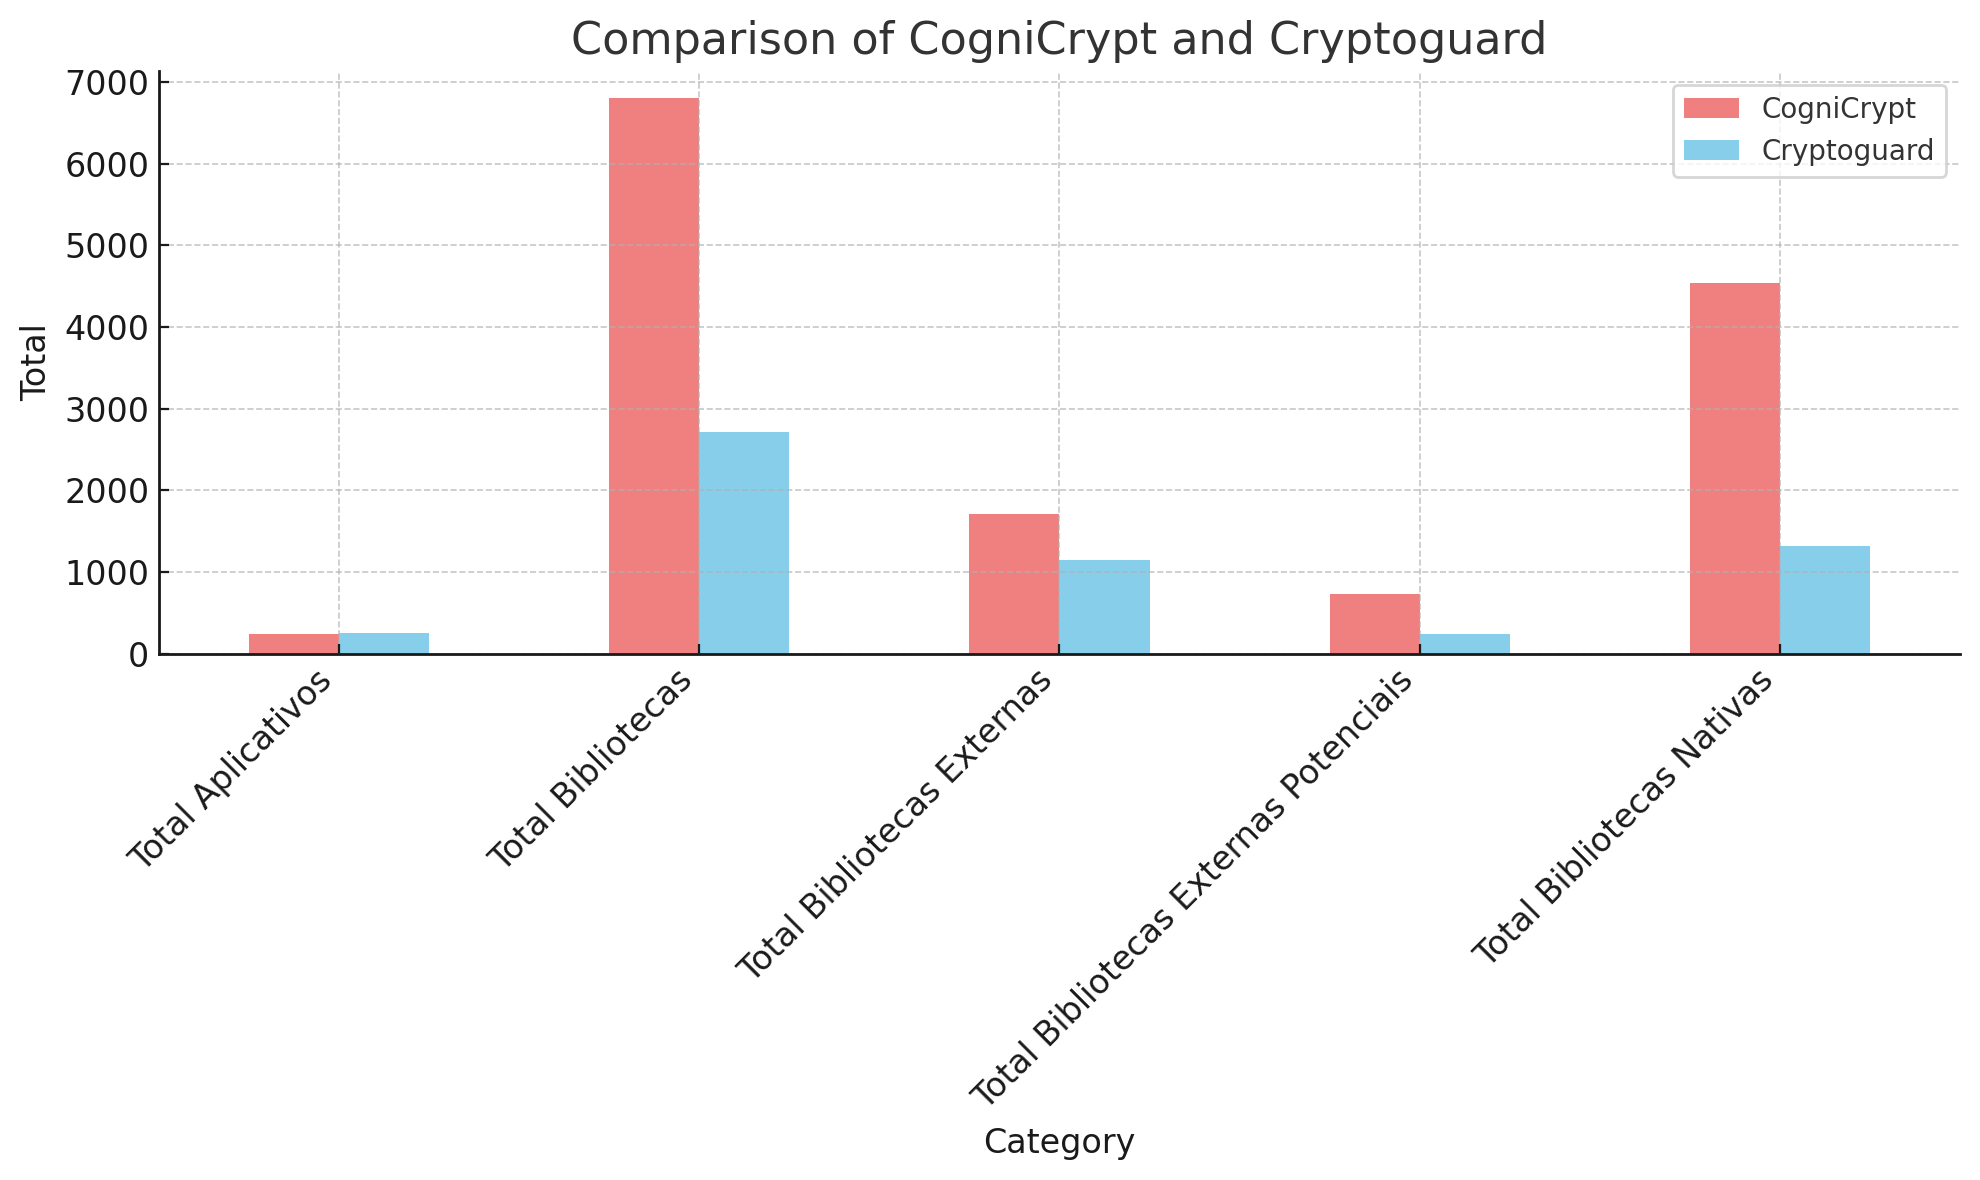
\includegraphics[scale=0.7]{img/plot_cc_x_cg_summary.png}
  \caption{Comparação total entre as ferramentas CogniCrypt e CryptoGuard}
  \label{img: CCvsCG_Summary}
\end{figure}

\FloatBarrier

\begin{figure}[!ht]
  \centering
  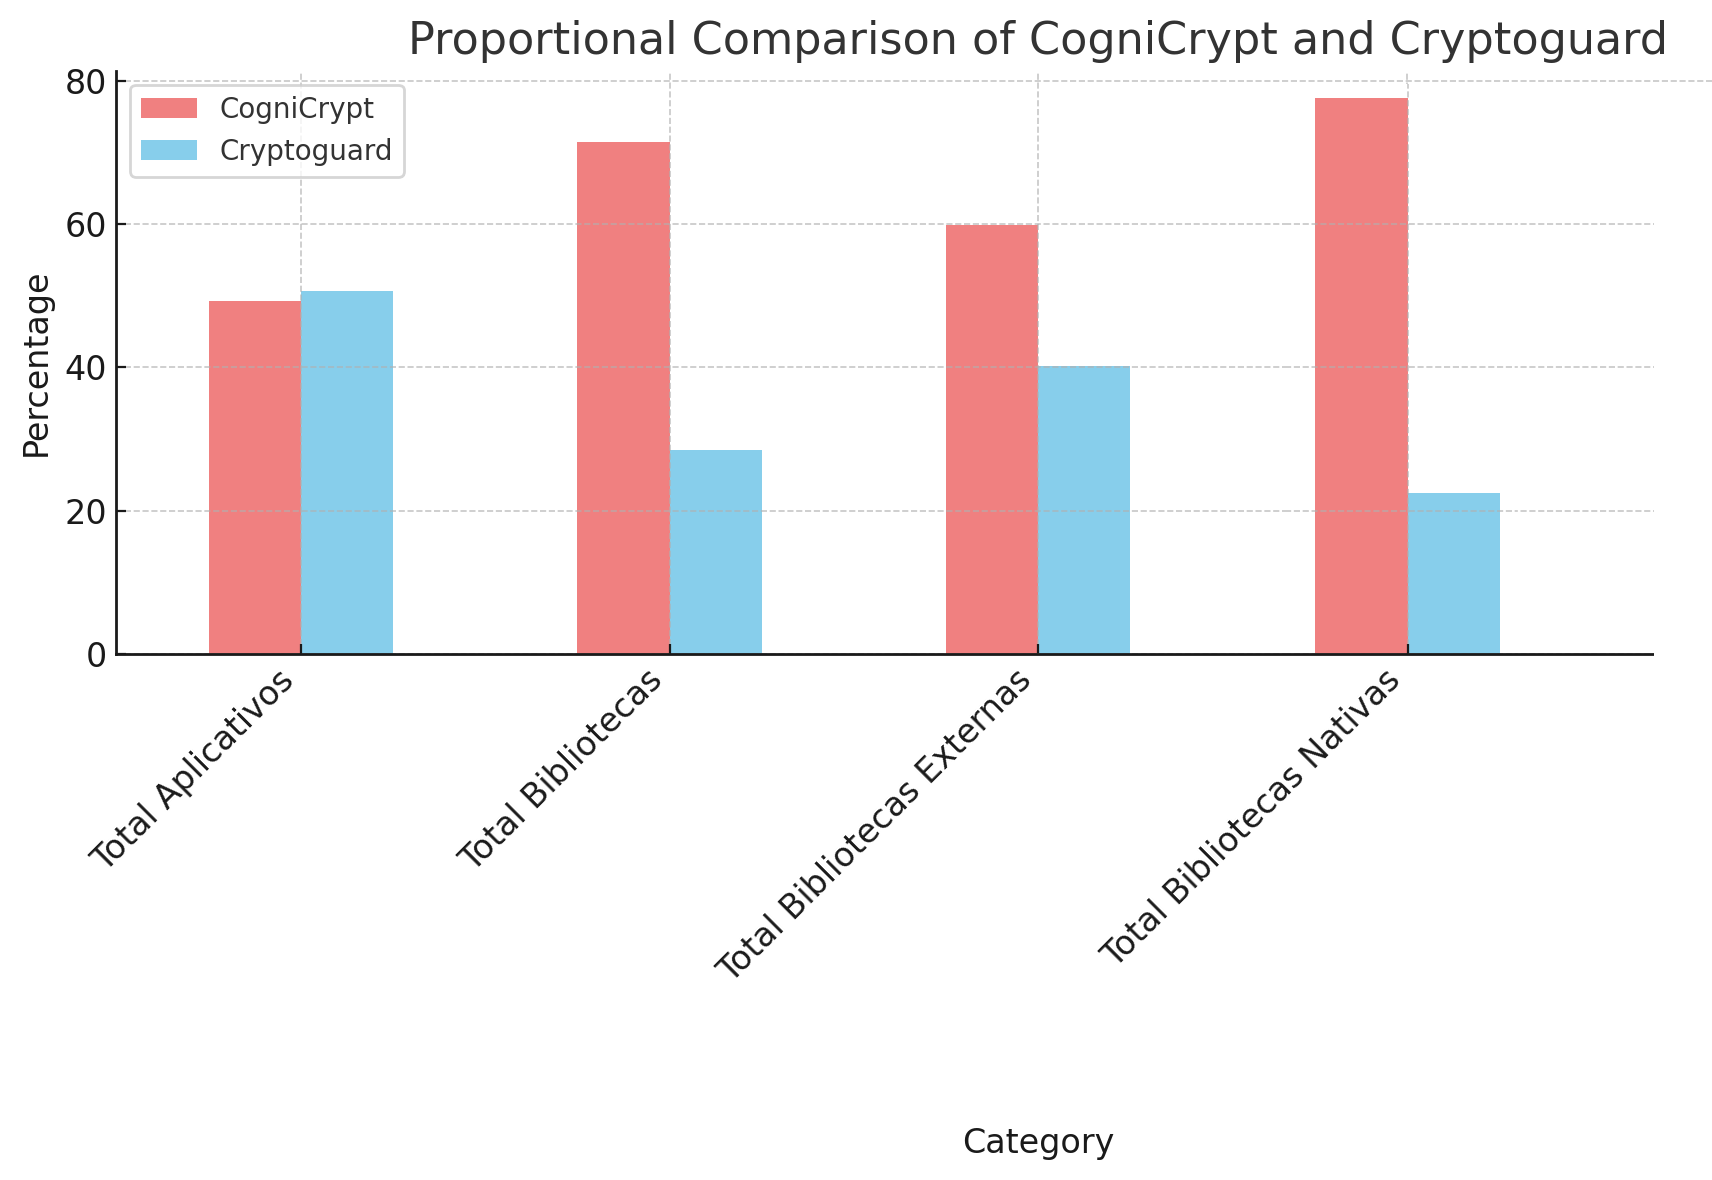
\includegraphics[scale=0.7]{img/plot_cc_x_cg_proportion_summary.png}
  \caption{Comparação proporcional total entre as ferramentas CogniCrypt e CryptoGuard}
  \label{img: CCvsCG_Summary2}
\end{figure}

\FloatBarrier

\begin{figure}[!ht]
  \centering
  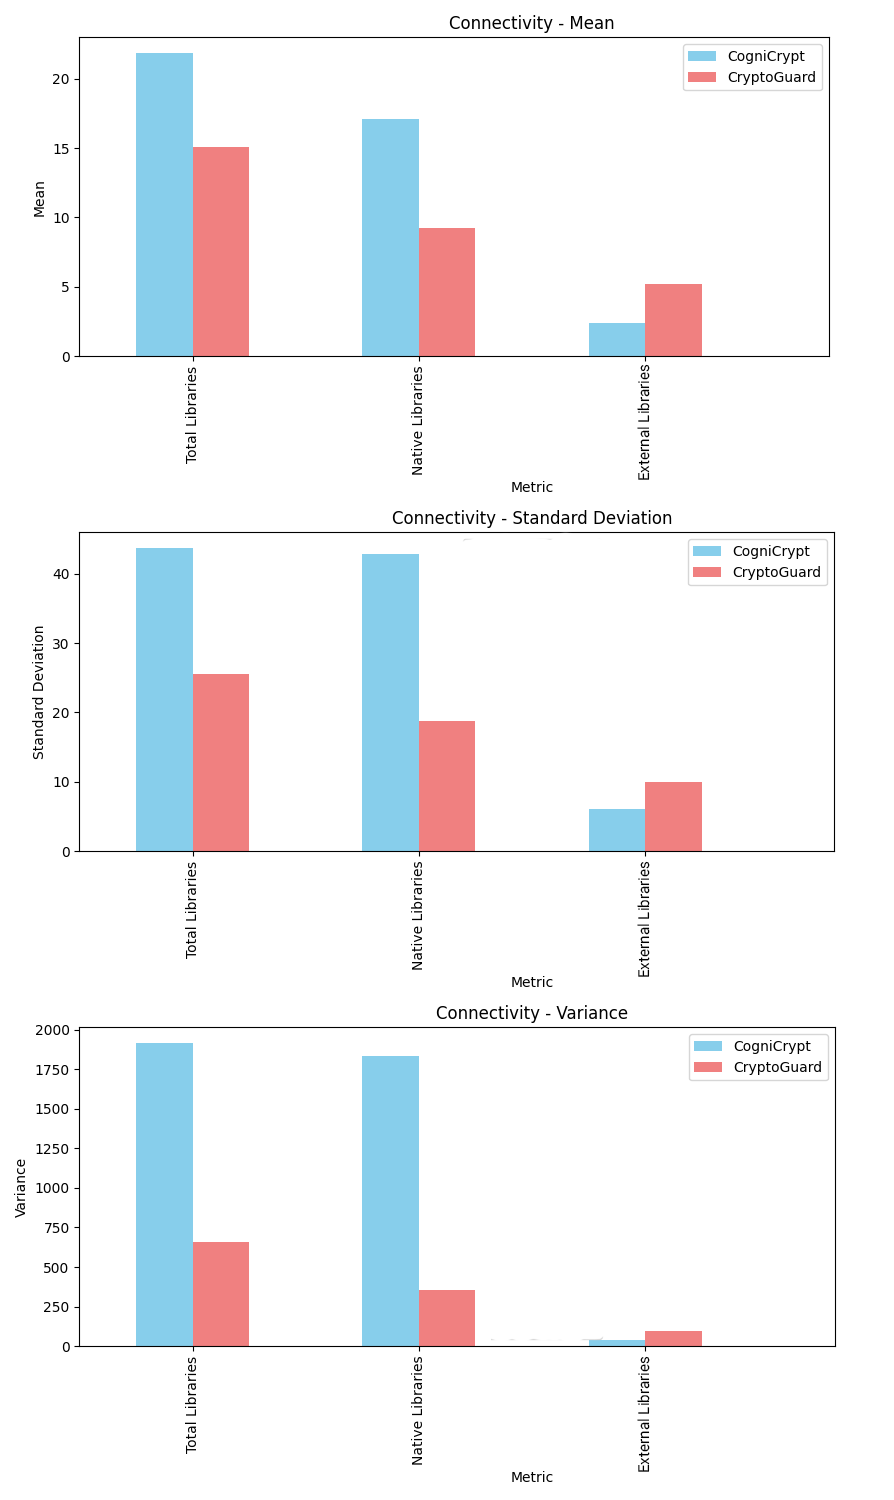
\includegraphics[scale=0.6]{img/plot_cc_x_cg_connectivity.png}
  \caption{Comparação entre as ferramentas CogniCrypt e CryptoGuard na categoria Connectivity}
  \label{img: CCvsCG_Connectivity}
\end{figure}

\FloatBarrier

\begin{figure}[!ht]
    \centering
    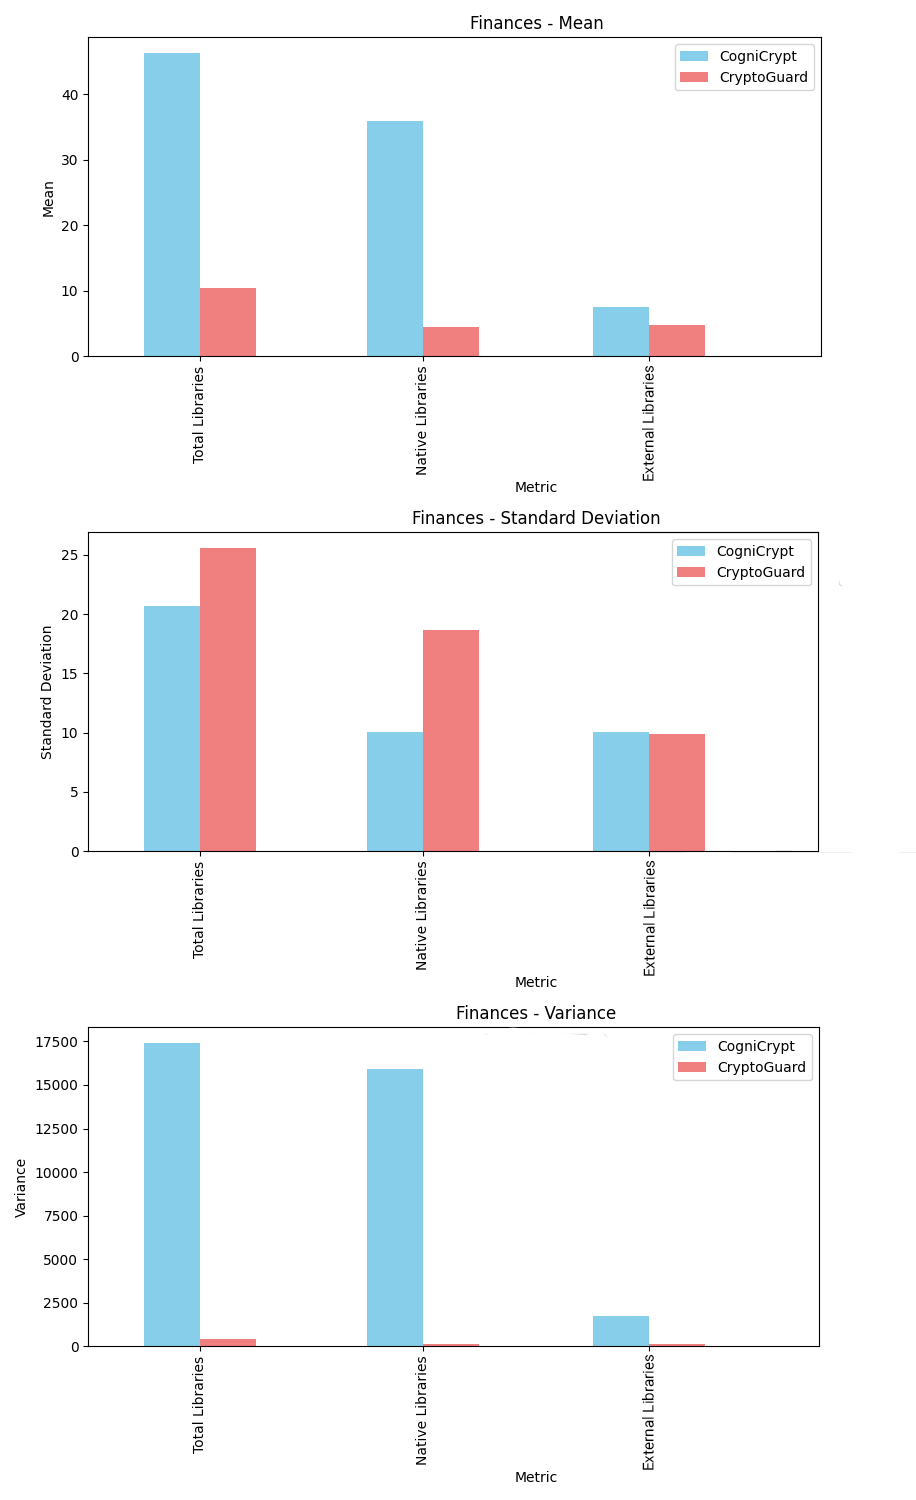
\includegraphics[scale=0.6]{img/plot_cc_x_cg_finances.png}
    \caption{Comparação entre as ferramentas CogniCrypt e CryptoGuard na categoria Finances}
    \label{img: CCvsCG_Finances}
\end{figure}

\FloatBarrier

\begin{figure}[!ht]
    \centering
    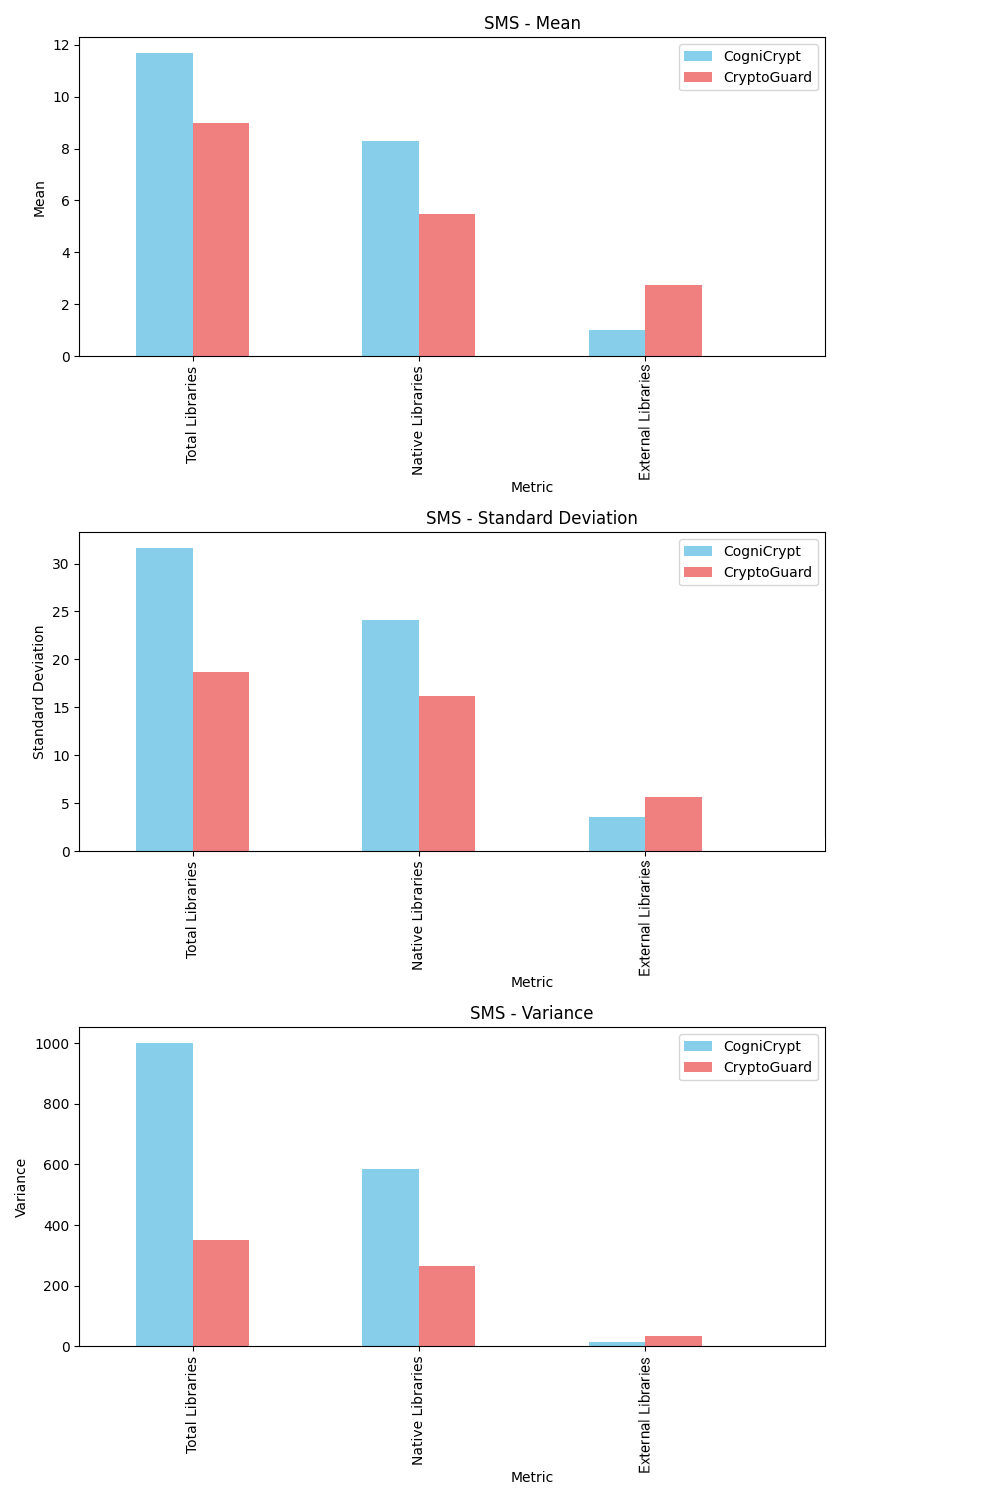
\includegraphics[scale=0.6]{img/plot_cc_x_cg_sms.png}
    \caption{Comparação entre as ferramentas CogniCrypt e CryptoGuard na categoria SMS}
    \label{img: CCvsCG_SMS}
\end{figure}

\FloatBarrier

\begin{figure}[!ht]
    \centering
    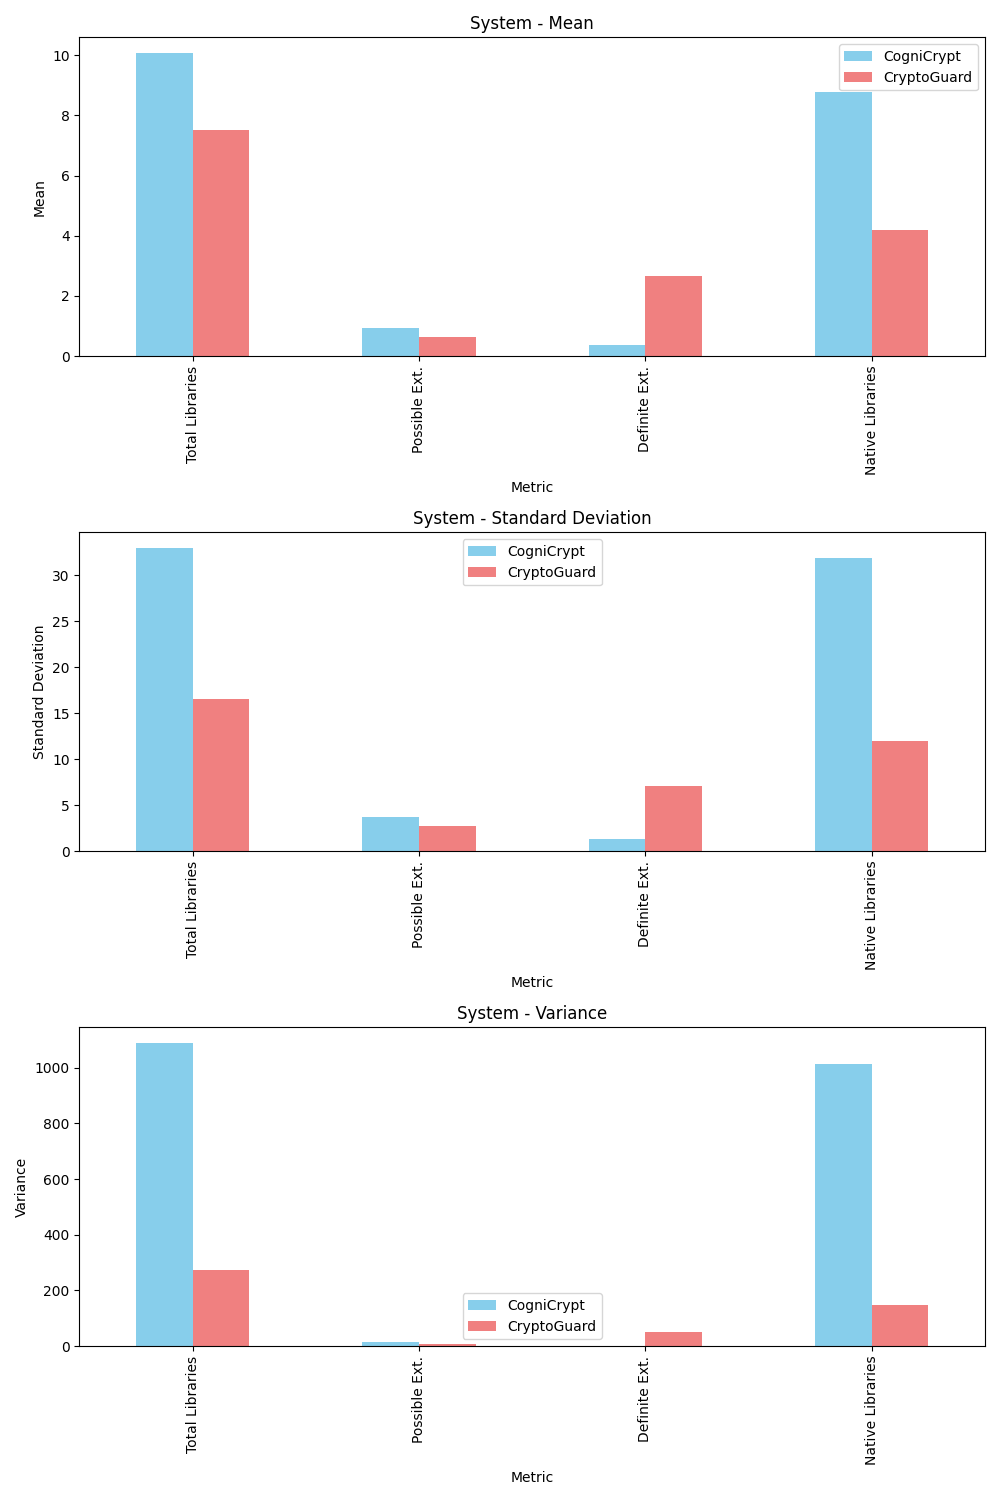
\includegraphics[scale=0.6]{img/plot_cc_x_cg_system.png}
    \caption{Comparação entre as ferramentas CogniCrypt e CryptoGuard na categoria System}
    \label{img: CCvsCG_System}
\end{figure}


\FloatBarrier


\begin{figure}[!ht]
  \centering
  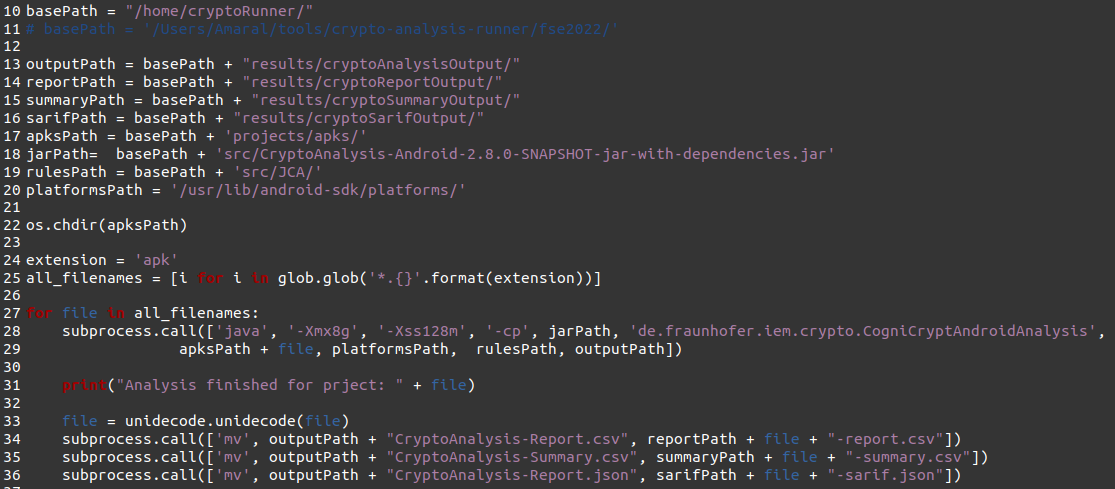
\includegraphics[scale=0.4]{img/cognicrypt_script.png}
  \caption{Script utilizado para rodar o CogniCrypt}
  \label{img: cognicrypt_script}
\end{figure}

\FloatBarrier

\begin{figure}[!ht]
  \centering
  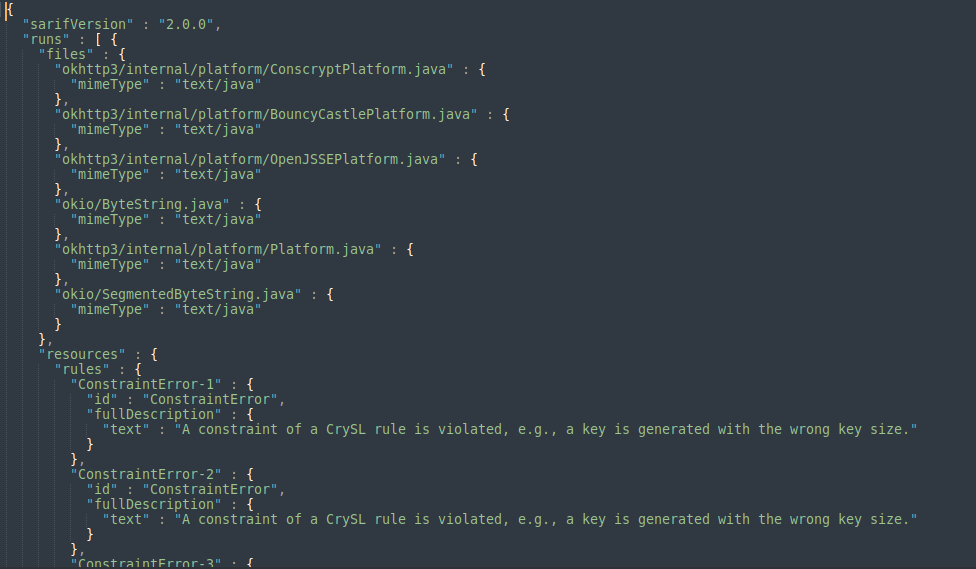
\includegraphics[scale=0.5]{img/cognicrypt_output.png}
  \caption{Output da ferramenta Cognicrypt para o apk Ademar.bitac\_5}
  \label{img: cognicrypt_output}
\end{figure}

\FloatBarrier

\begin{figure}[!ht]
  \centering
  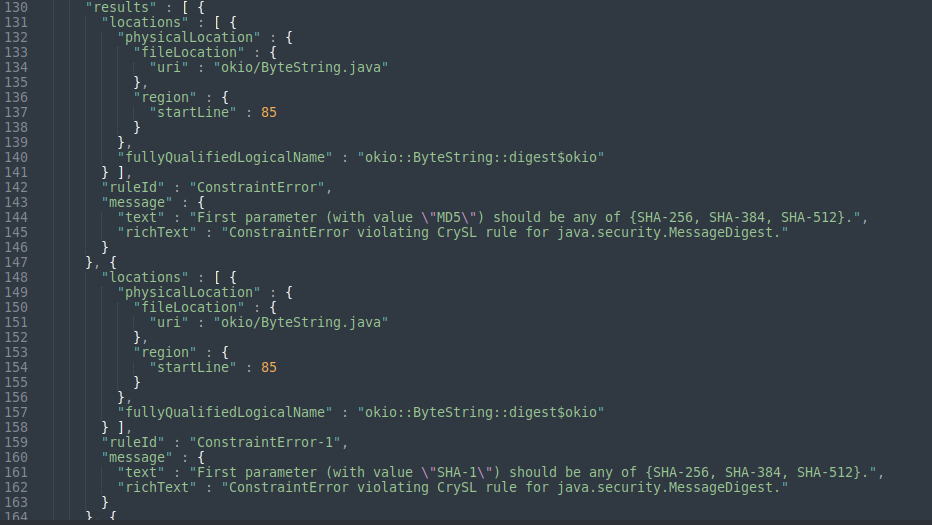
\includegraphics[scale=0.5]{img/cognicrypt_output2.png}
  \caption{Output da ferramenta Cognicrypt para o apk Ademar.bitac\_5}
  \label{img: cognicrypt_output2}
\end{figure}

\FloatBarrier

\begin{figure}[!ht]
  \centering
  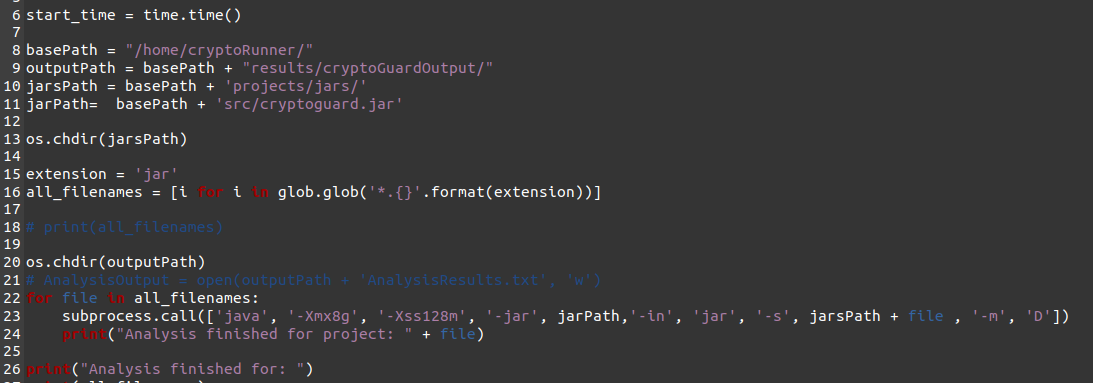
\includegraphics[scale=0.4]{img/cryptoguard_script.png}
  \caption{Script utilizado para rodar o CryptoGuard}
  \label{img: cryptoguard_script}
\end{figure}

\FloatBarrier

\begin{figure}[!ht]
  \centering
  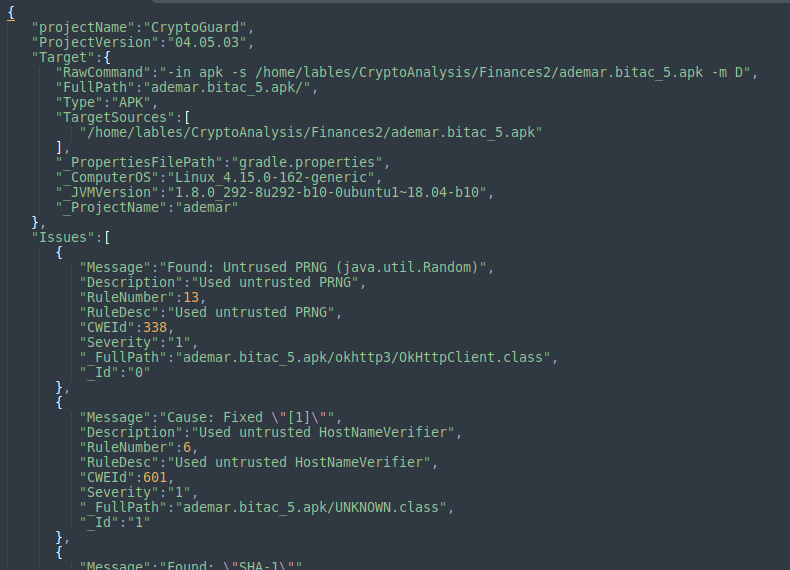
\includegraphics[scale=0.5]{img/cryptoguard_output.png}
  \caption{Output da ferramenta Cryptoguard para o apk Ademar.bitac\_5}
  \label{img: cryptoguard_output}
\end{figure}

\FloatBarrier


\begin{figure}[!ht]
  \centering
  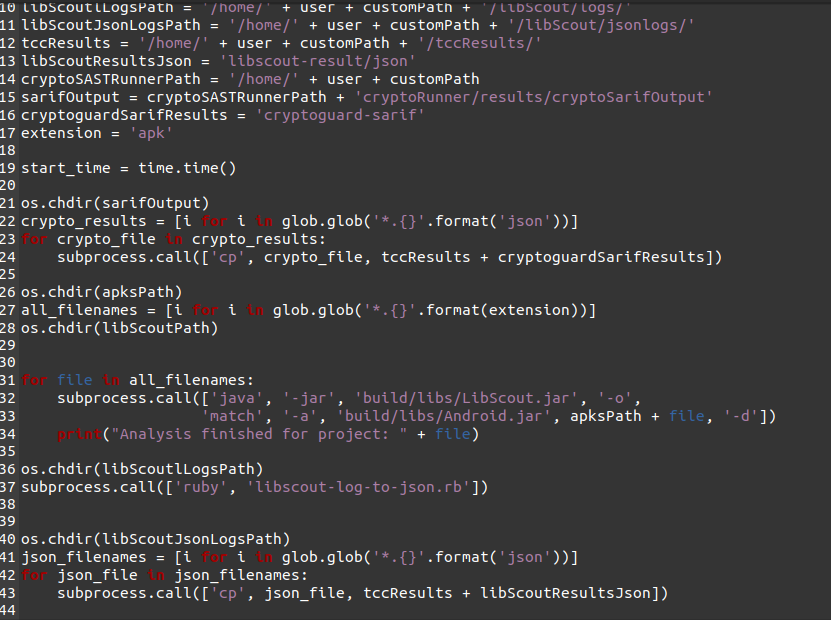
\includegraphics[scale=0.5]{img/libscout_script.png}
  \caption{Script utilizado para rodar o LibScout}
  \label{img: libscout_script}
\end{figure}

\FloatBarrier

\begin{figure}[!ht]
  \centering
  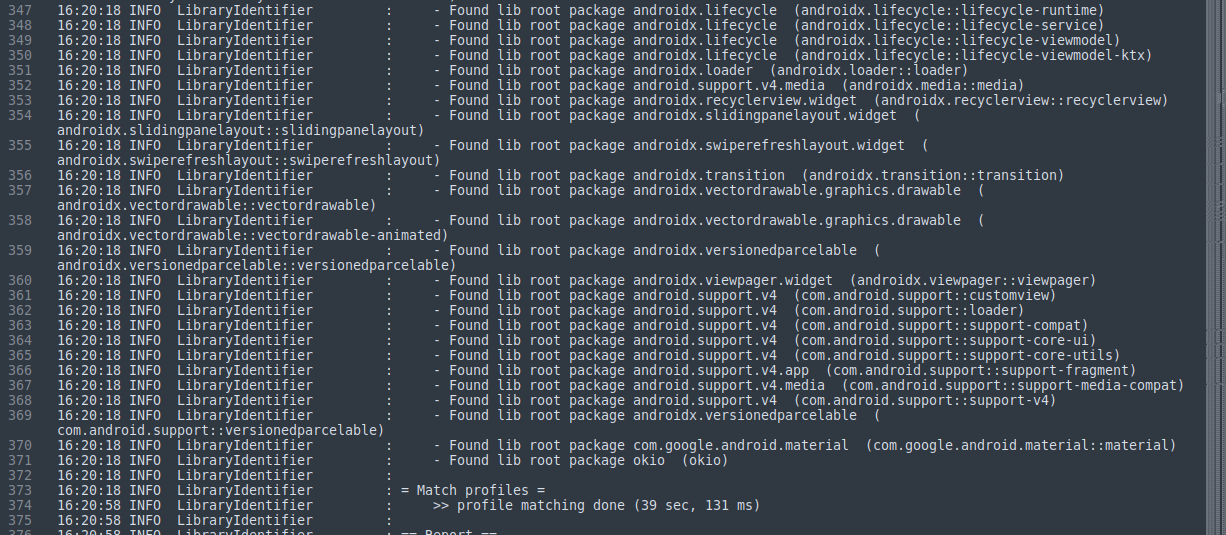
\includegraphics[scale=0.4]{img/libscout_output.png}
  \caption{Output da ferramenta LibScout para o apk Ademar.bitac\_5}
  \label{img: libscout_output}
\end{figure}

\FloatBarrier

\begin{figure}[!ht]
  \centering
  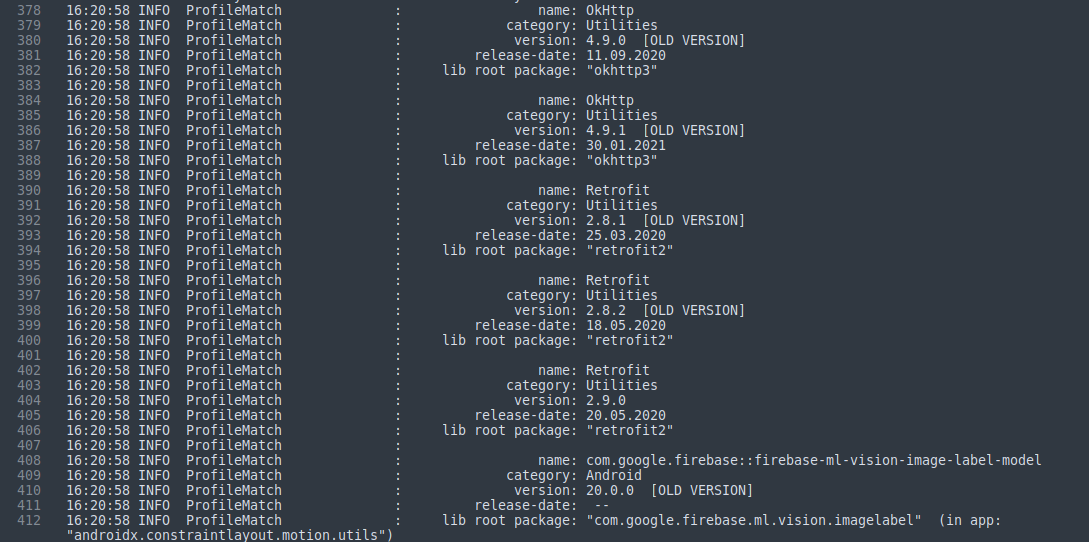
\includegraphics[scale=0.4]{img/libscout_output2.png}
  \caption{Output da ferramenta LibScout para o apk Ademar.bitac\_5}
  \label{img: libscout_output2}
\end{figure}

\FloatBarrier

\begin{figure}[!ht]
  \centering
  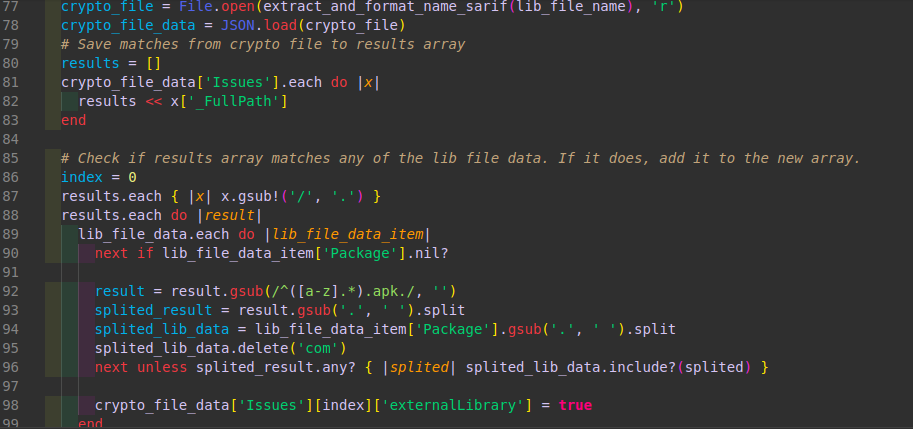
\includegraphics[scale=0.5]{img/integration_script_cogni.png}
  \caption{Script utilizado para integrar os resultados do LibScout com os resultados do CogniCrypt}
  \label{img: integration_script_cogni}
\end{figure}

\FloatBarrier

\begin{figure}[!ht]
  \centering
  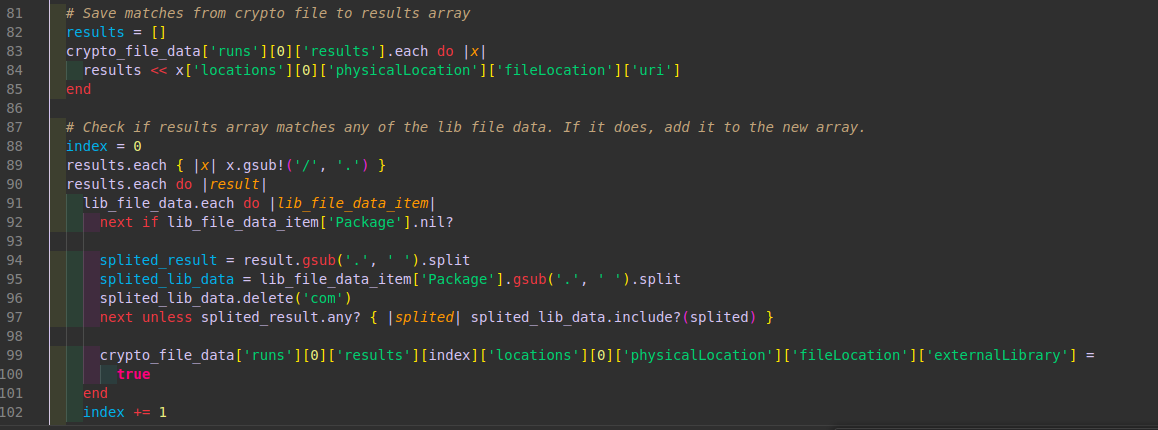
\includegraphics[scale=0.4]{img/integration_script_crypto.png}
  \caption{Script utilizado para integrar os resultados do LibScout com os resultados do CryptoGuard}
  \label{img: integration_script_crypto}
\end{figure}

\FloatBarrier


\begin{figure}[!ht]
  \centering
  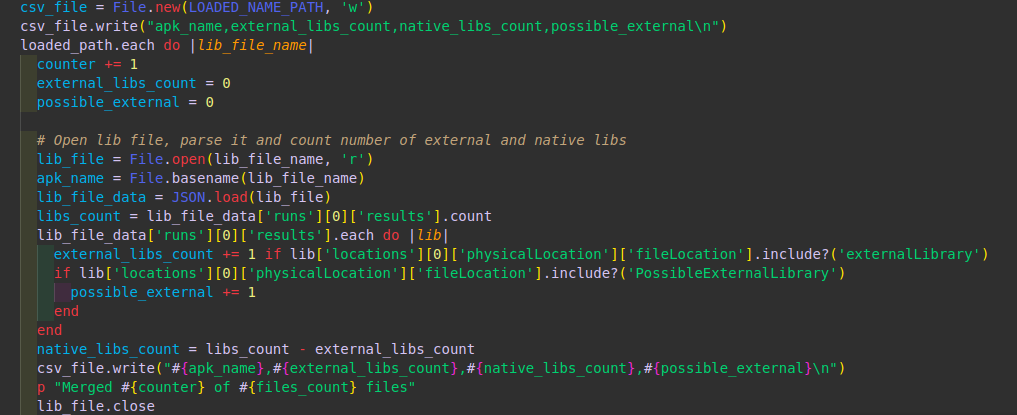
\includegraphics[scale=0.5]{img/output_script_counter.png}
  \caption{Script utilizado para gerar os arquivos de saída para análise}
  \label{img: output_script}
\end{figure}

\FloatBarrier